\section{Motivating example: Pairs of applications}
\label{sec:motivation}
We assume we have a set of applications $S$ with $\|S\| = m$ applications. Each of the applications have to finish work of amount $w_1, w_2,. . . w_m$. They can be scheduled to run alone or with other applications. When application i is run alone it runs with speed $r_{ii}$, when its run with another application j, it runs with $r_{ij}$. What is the fastest schedule to complete all the jobs of the application? Assume $r_{ii} > r_{ij}$ for all $i$. We observe that for every schedule we can draw an undirected graph with nodes being the application and the edge weight between node $i$ and node $j$ indicates that the application i is run with application $j$ for time $t_{ij}$. Similarly, for every graph which does  not contain cycle and (other constraint on path from each node), we can find a schedule. Note that self edges are allowed which means the application is run alone for some time indicated by the weight on the self edge. Hence we want to find a graph with minimum sum of edge weight which finishes the work by all applications. We describe a linear program for optimal scheduling.

\begin{figure*}[htp!]
\begin{center}
 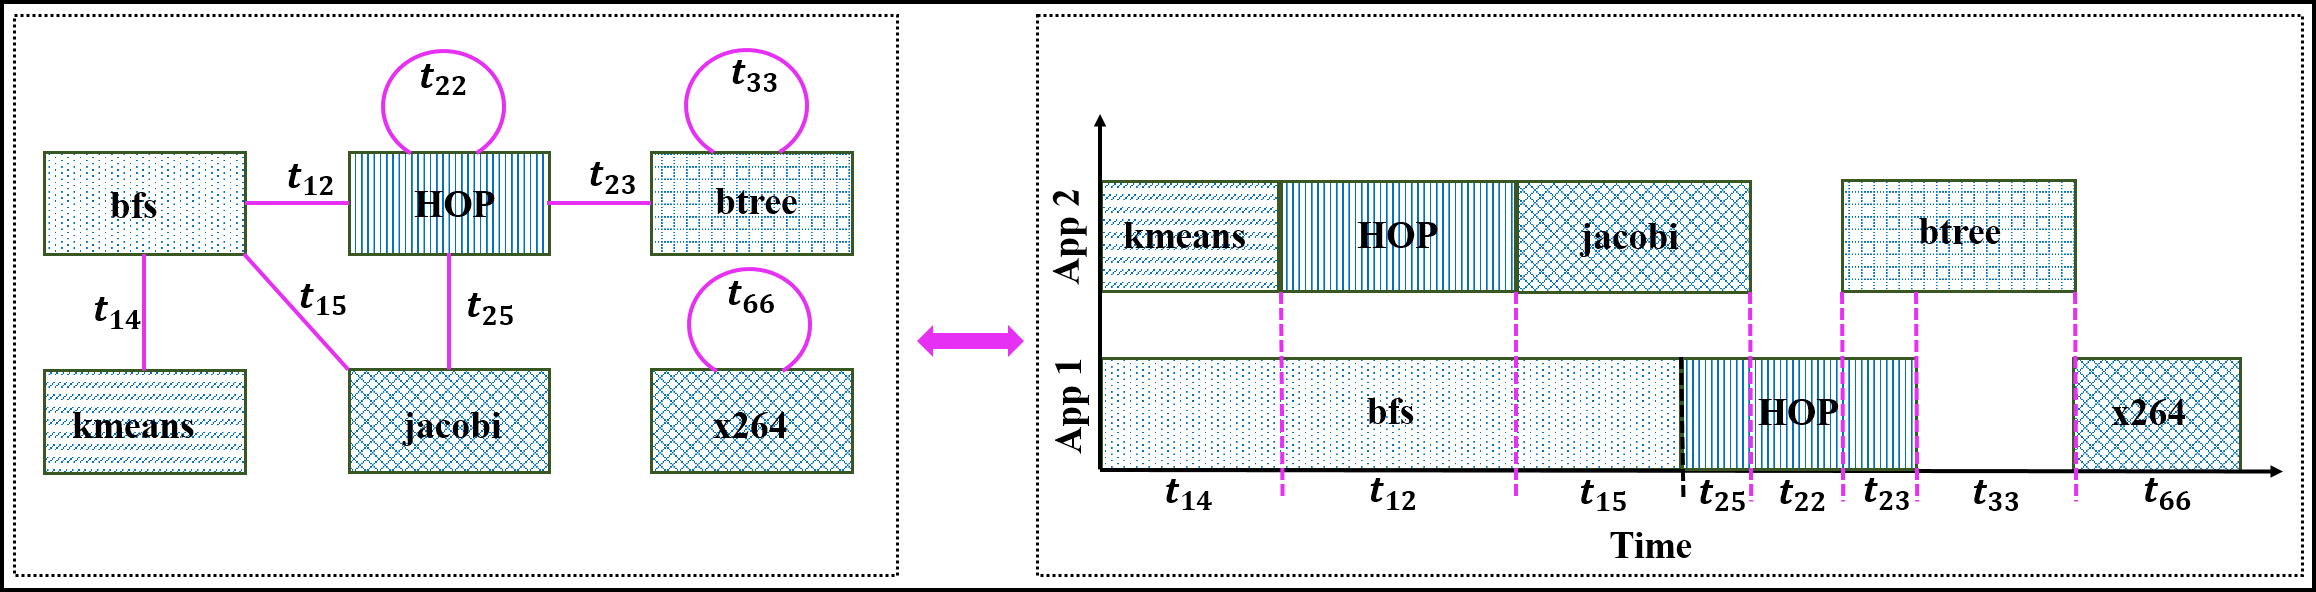
\includegraphics[width=1\textwidth]{figures/PairGraphSchedulebp.png}
  \caption{  Graph.}
\label{fig:simulation}
\end{center}
\end{figure*}


\begin{enumerate}
\item Comparison,
\begin{enumerate}
\item Baseline is the eurosys paper. We have modified it to include work.
\begin{enumerate}
\item memory
\item IPC
\item L3 cache requests
\end{enumerate}
\item First come first served(random).

\item Optimal algorithm with measurement noise.(100 samples)
\end{enumerate}
\PUNT{
\begin{figure}[h]
\begin{center}
 \includegraphics[width=0.5\textwidth]{../figures/main_pair_AllBaseline.png}
  \caption{  Simulation results.}
\label{fig:simulation}
\end{center}
\end{figure}
}

\item Classification: To combine or not

\PUNT{
\begin{figure}[h]
\begin{center}
 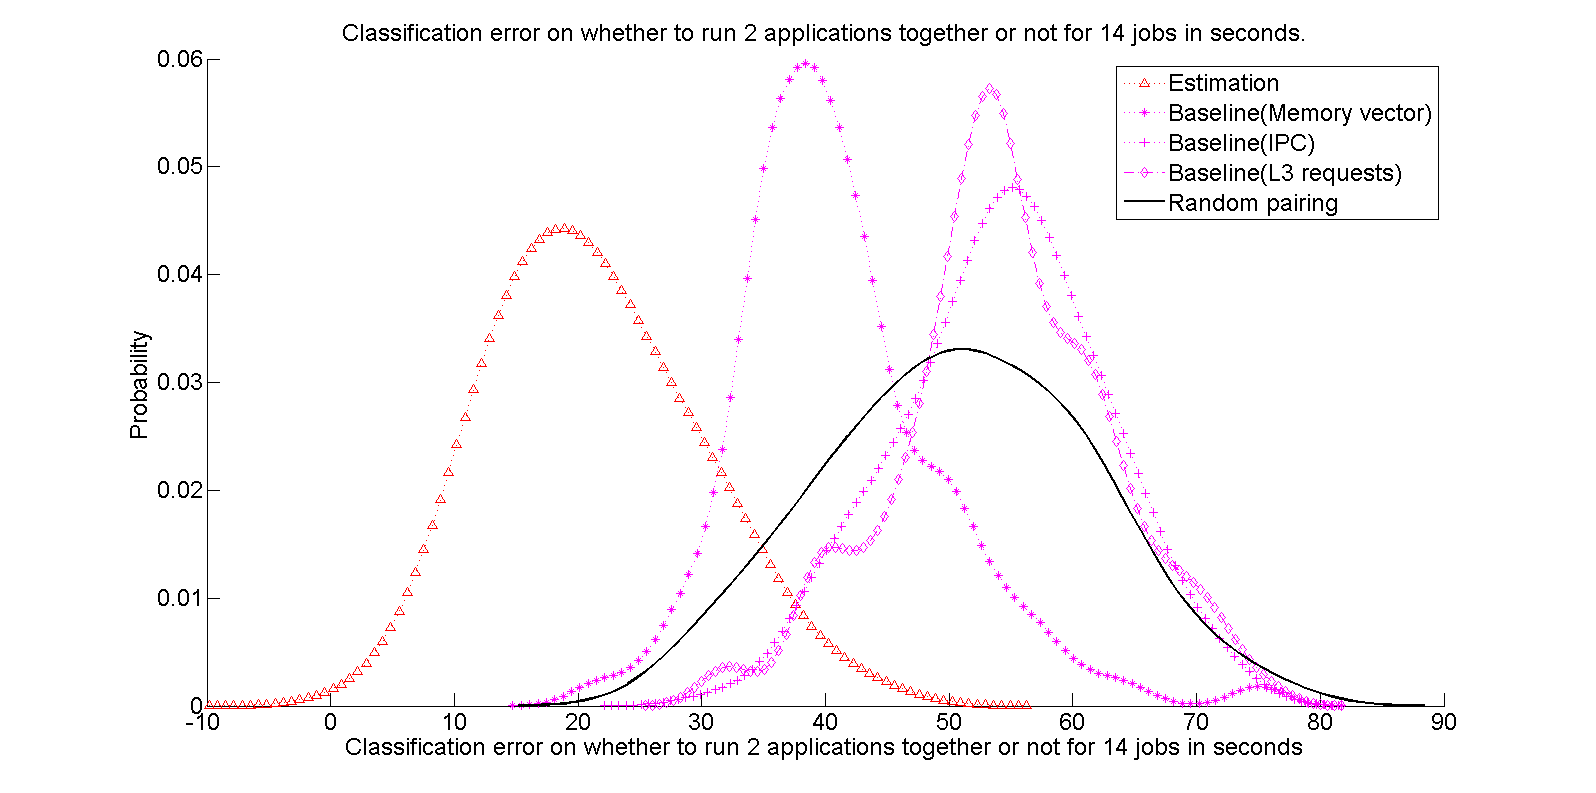
\includegraphics[width=0.5\textwidth]{../figures/Clsf.png}
  \caption{  Simulation results.}
\label{fig:simulation}
\end{center}
\end{figure}
}

We are optimizing the threshold for each baseline. Its essentially a binary tree kind of classification for individual low level features with best threshold. The classification error is averaged over 100 samples.
\end{enumerate}

Linear program for pairs of applications.
\begin{equation}
\begin{aligned}
\label{eq:pairschedule}
&   \underset{T \geq 0}{\text{min}}  
&&   \sum_{i \geq j} \sum_{j=1:m} T_{ij} \\
&   \text{subject to} &&  \sum_{j=1:m} R_{ij} T_{ij} = w_i, \quad  \forall i\in [m],\\
&&&	  T_{ij} = T_{ji}, \quad \forall i,j \in [m].\\
\end{aligned}
\end{equation}

\PUNT{
Transformation to CVX linear program,

\begin{equation}
\begin{aligned}
\label{eq:controller}
&   \underset{T}{\text{min}}  
&&  \tr( \text{triu}(\text{ones}(m)) T)=\tr( B T) \\
&   \text{subject to} &&  \diag( R T) = w,\\
&&&	  T = T',\\
&&&	  T \geq 0.\\
\end{aligned}
\end{equation}
}